\section{tasks::ordermerge Class Reference}
\label{classtasks_1_1ordermerge}\index{tasks::ordermerge@{tasks::ordermerge}}
Inheritance diagram for tasks::ordermerge::\begin{figure}[H]
\begin{center}
\leavevmode
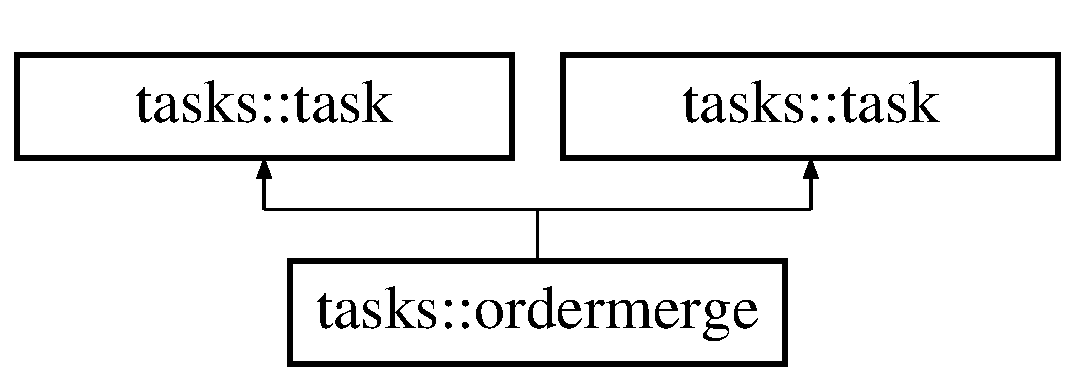
\includegraphics[height=2cm]{classtasks_1_1ordermerge}
\end{center}
\end{figure}
\subsection*{Public Member Functions}
\begin{CompactItemize}
\item 
def \textbf{run}\label{classtasks_1_1ordermerge_735e8002c7420e551a051304d39ecce7}

\item 
def \textbf{run}\label{classtasks_1_1ordermerge_735e8002c7420e551a051304d39ecce7}

\end{CompactItemize}
\subsection*{Static Public Attributes}
\begin{CompactItemize}
\item 
string \textbf{name} = '{\bfordermerge}'\label{classtasks_1_1ordermerge_38bb09d69dd62d1cfbcb3846e7a9363e}

\item 
string \textbf{button\-Text} = 'Merge orders'\label{classtasks_1_1ordermerge_70658f63557c39e40122709254557c0c}

\item 
string \textbf{suffix} = 'merge'\label{classtasks_1_1ordermerge_22921dd8fc1f820c81b37205ab9a0a7d}

\item 
list \textbf{prereq} = ['{\bfblazecorr}', '{\bfaddwave}']\label{classtasks_1_1ordermerge_ab46b0b2a63158eb3cca9d547c775852}

\end{CompactItemize}


\subsection{Detailed Description}


\footnotesize\begin{verbatim}Merge extracted orders into one 1-dimensional spectrum. Because the wavelength
   grid of the individual orders may be different, merging implies rebinning
   of the spectrum.
\end{verbatim}
\normalsize
 



The documentation for this class was generated from the following files:\begin{CompactItemize}
\item 
old/PANICtool-1.0/tasks.py\item 
old/tasks.py\end{CompactItemize}
